\subsection{Overview}
    \begin{frame}
        \frametitle{Overview}
        \textbf{Additive manufacturing has the potential to radically transform reactor design.}
        \vspace{0.5cm}

        In this defense, I will show that I successfully: 
        \begin{enumerate}
            \item Furthered our understanding of the \gls{AHTR} design's complexities 
            through neutronics and thermal-hydraulics modeling
            \item Created an open-source tool that enables reactor generative 
            design optimization for non-conventional geometries and fuel 
            distributions with evolutionary algorithms
            \item Applied the optimization tool to the \gls{AHTR} design 
        \end{enumerate}
    \end{frame}

\subsection{Background: Advanced High Temperature Reactor}
    \begin{frame}
        \frametitle{Why Generation IV Reactors?}
        \begin{itemize}
        \item Energy use and production contribute $\frac{2}{3}$ of Greenhouse Gas 
        emissions \cite{noauthor_climate_2018}
        \item  Large scale emissions-free nuclear power deployment could 
        significantly reduce GHG production but faces both cost and perceived 
        safety challenges 
        \item The Generation IV International Forum identified six systems 
        that promise significant advances in safety, sustainability, efficiency, 
        and cost over existing designs: GFR, LFR, MSR, SFR, SCWR, and VHTR. 
        \begin{figure}[htbp!]
            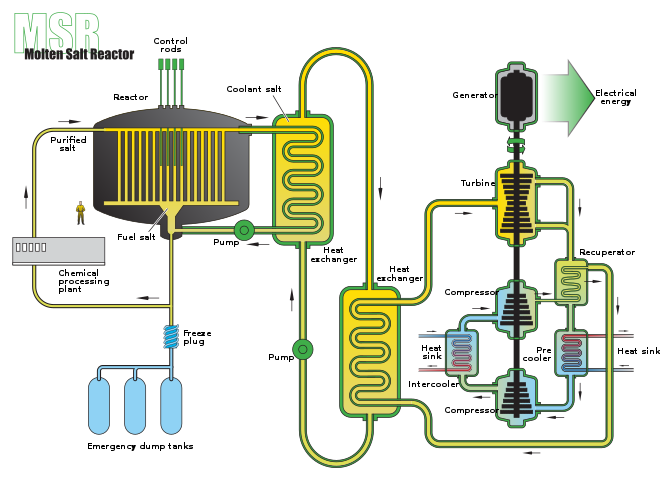
\includegraphics[height=3cm]{figures/msr}
            \hspace{1cm}
            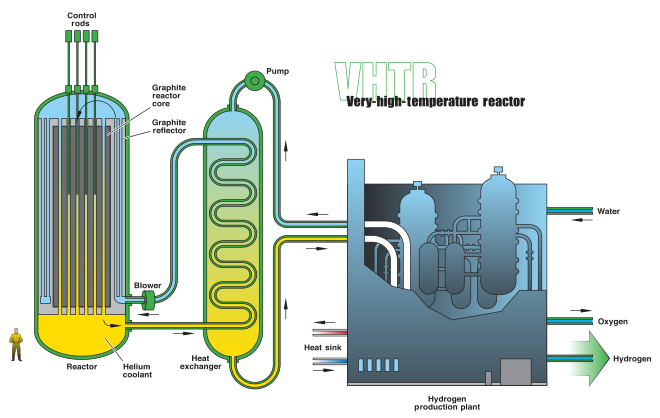
\includegraphics[height=3cm]{figures/vhtr}
            \caption{Left: Molten Salt Reactor System, Right: Very High-Temperature
            Reactor System \cite{gif_technology_2002}. }
        \end{figure}
        \end{itemize}
    \end{frame}
    \begin{frame}
    \frametitle{MSRs and VHTRs}
    \begin{block}{Molten Salt Reactor (MSR) System Advantages}
        \begin{itemize}
        \item Molten Fluoride Salts: chemical stability, low vapor pressure at 
        high temperatures, good heat transfer, resistance against radiation damage
        \item Inherent System Safety: passive cooling, fail-safe drainage
        \end{itemize}
    \end{block}
    \vspace{-0.25cm}
    \begin{block}{Very High Temperature Reactor (VHTR) System Advantages}
        \begin{itemize}
        \item TRISO Fuel: withstands high burnup and temperature
        \item High Outlet Temperature: increases power conversion efficiency, reduces 
        waste heat generation, enables high-temperature heat applications 
        \end{itemize}
    \end{block}
    \begin{figure}[htbp!]
        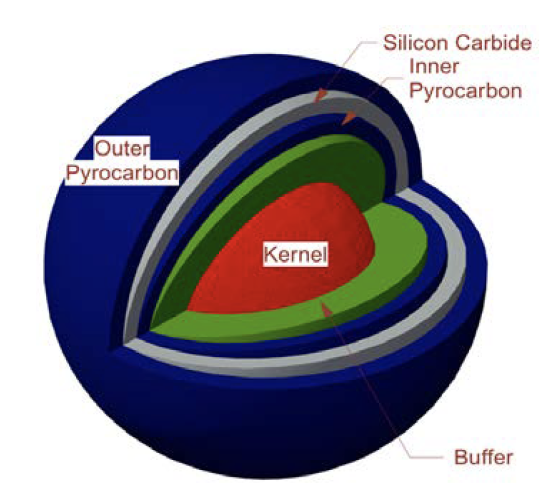
\includegraphics[width=0.2\linewidth]{../docs/figures/ahtr-triso.png}
        \caption{TRISO particle. Diameter: $\sim 8mm$}
    \end{figure}
    \end{frame}
    \begin{frame}
    \frametitle{\acrlong{FHR}}
    FHR concept combines the best aspects of MSR and VHTR:
    low-pressure liquid fluoride-salt coolant and TRISO fuel 
    \begin{block}{\acrfull{FHR} Advantages}
        \begin{itemize}
        \item Molten salt coolant vs. VHTR helium coolant: superior cooling, 
        moderating properties, low operating pressure, large thermal margin
        \item TRISO fuel vs. MSR circulating liquid fuel: solid fuel cladding 
        adds an extra barrier to fission product release
        \end{itemize}
    \end{block}
    \begin{figure}[]
        \centering
        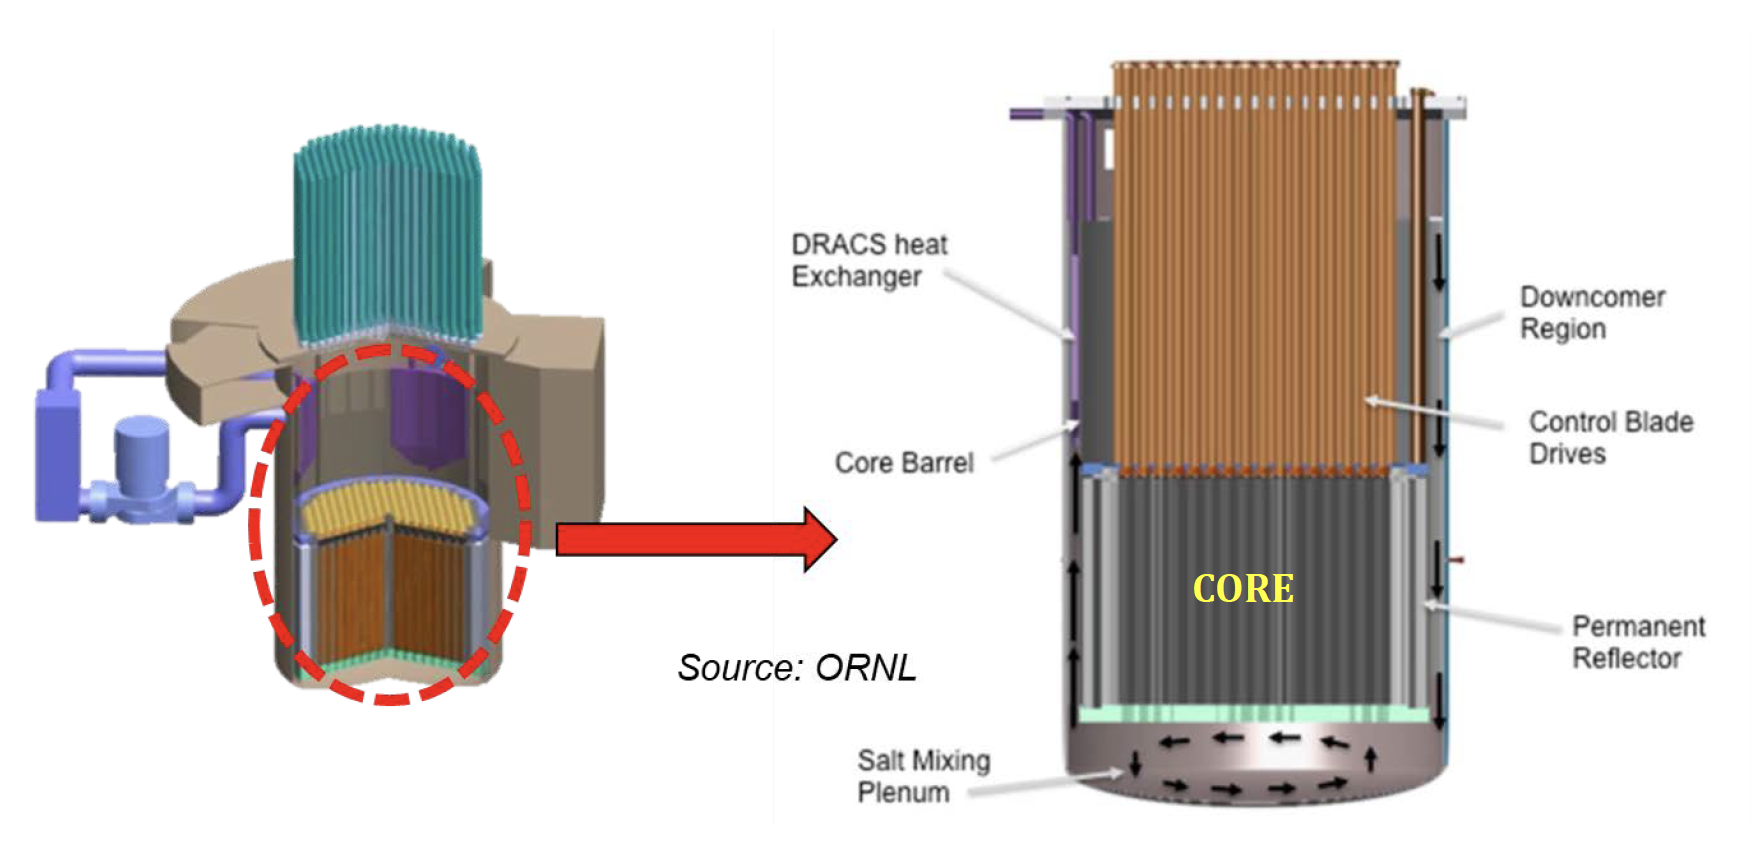
\includegraphics[width=0.5\linewidth]{../docs/figures/reactor-schematic.png} 
        \caption{\acrfull{AHTR} schematic (left) and vessel (right) reproduced from
        \cite{noauthor_fluoride_nodate}.}
    \end{figure}
    \end{frame}
    \begin{frame}
    \frametitle{Advanced High Temperature Reactor Design}
        \begin{itemize}
        \item Design developed by Oak Ridge National Laboratory
        \item Prismatic FHR design with 252 hexagonal fuel assemblies consisting of 
        18 fuel planks arranged in 3 diamond-shaped sectors. 
        \end{itemize}
    \begin{figure}[]
        \centering
        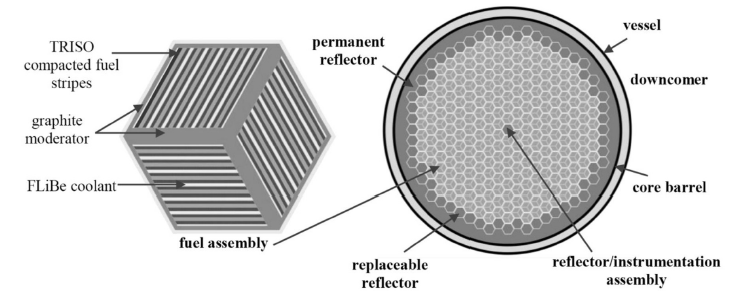
\includegraphics[width=0.9\linewidth]{../docs/figures/ahtr.png} 
        \caption{\acrlong{AHTR} fuel assembly (left) and core configuration (right) 
        reproduced from \cite{ramey_monte_2018}.}
        \label{fig:ahtr}
    \end{figure}
    \end{frame}

    \begin{frame}
    \frametitle{Advanced High Temperature Reactor Geometry}
    The AHTR fuel has a \emph{triple heterogeneity}: hexagonal fuel elements with 
    fuel planks, and TRISO particles embedded in stripes within each plank.
    \begin{figure}[]
        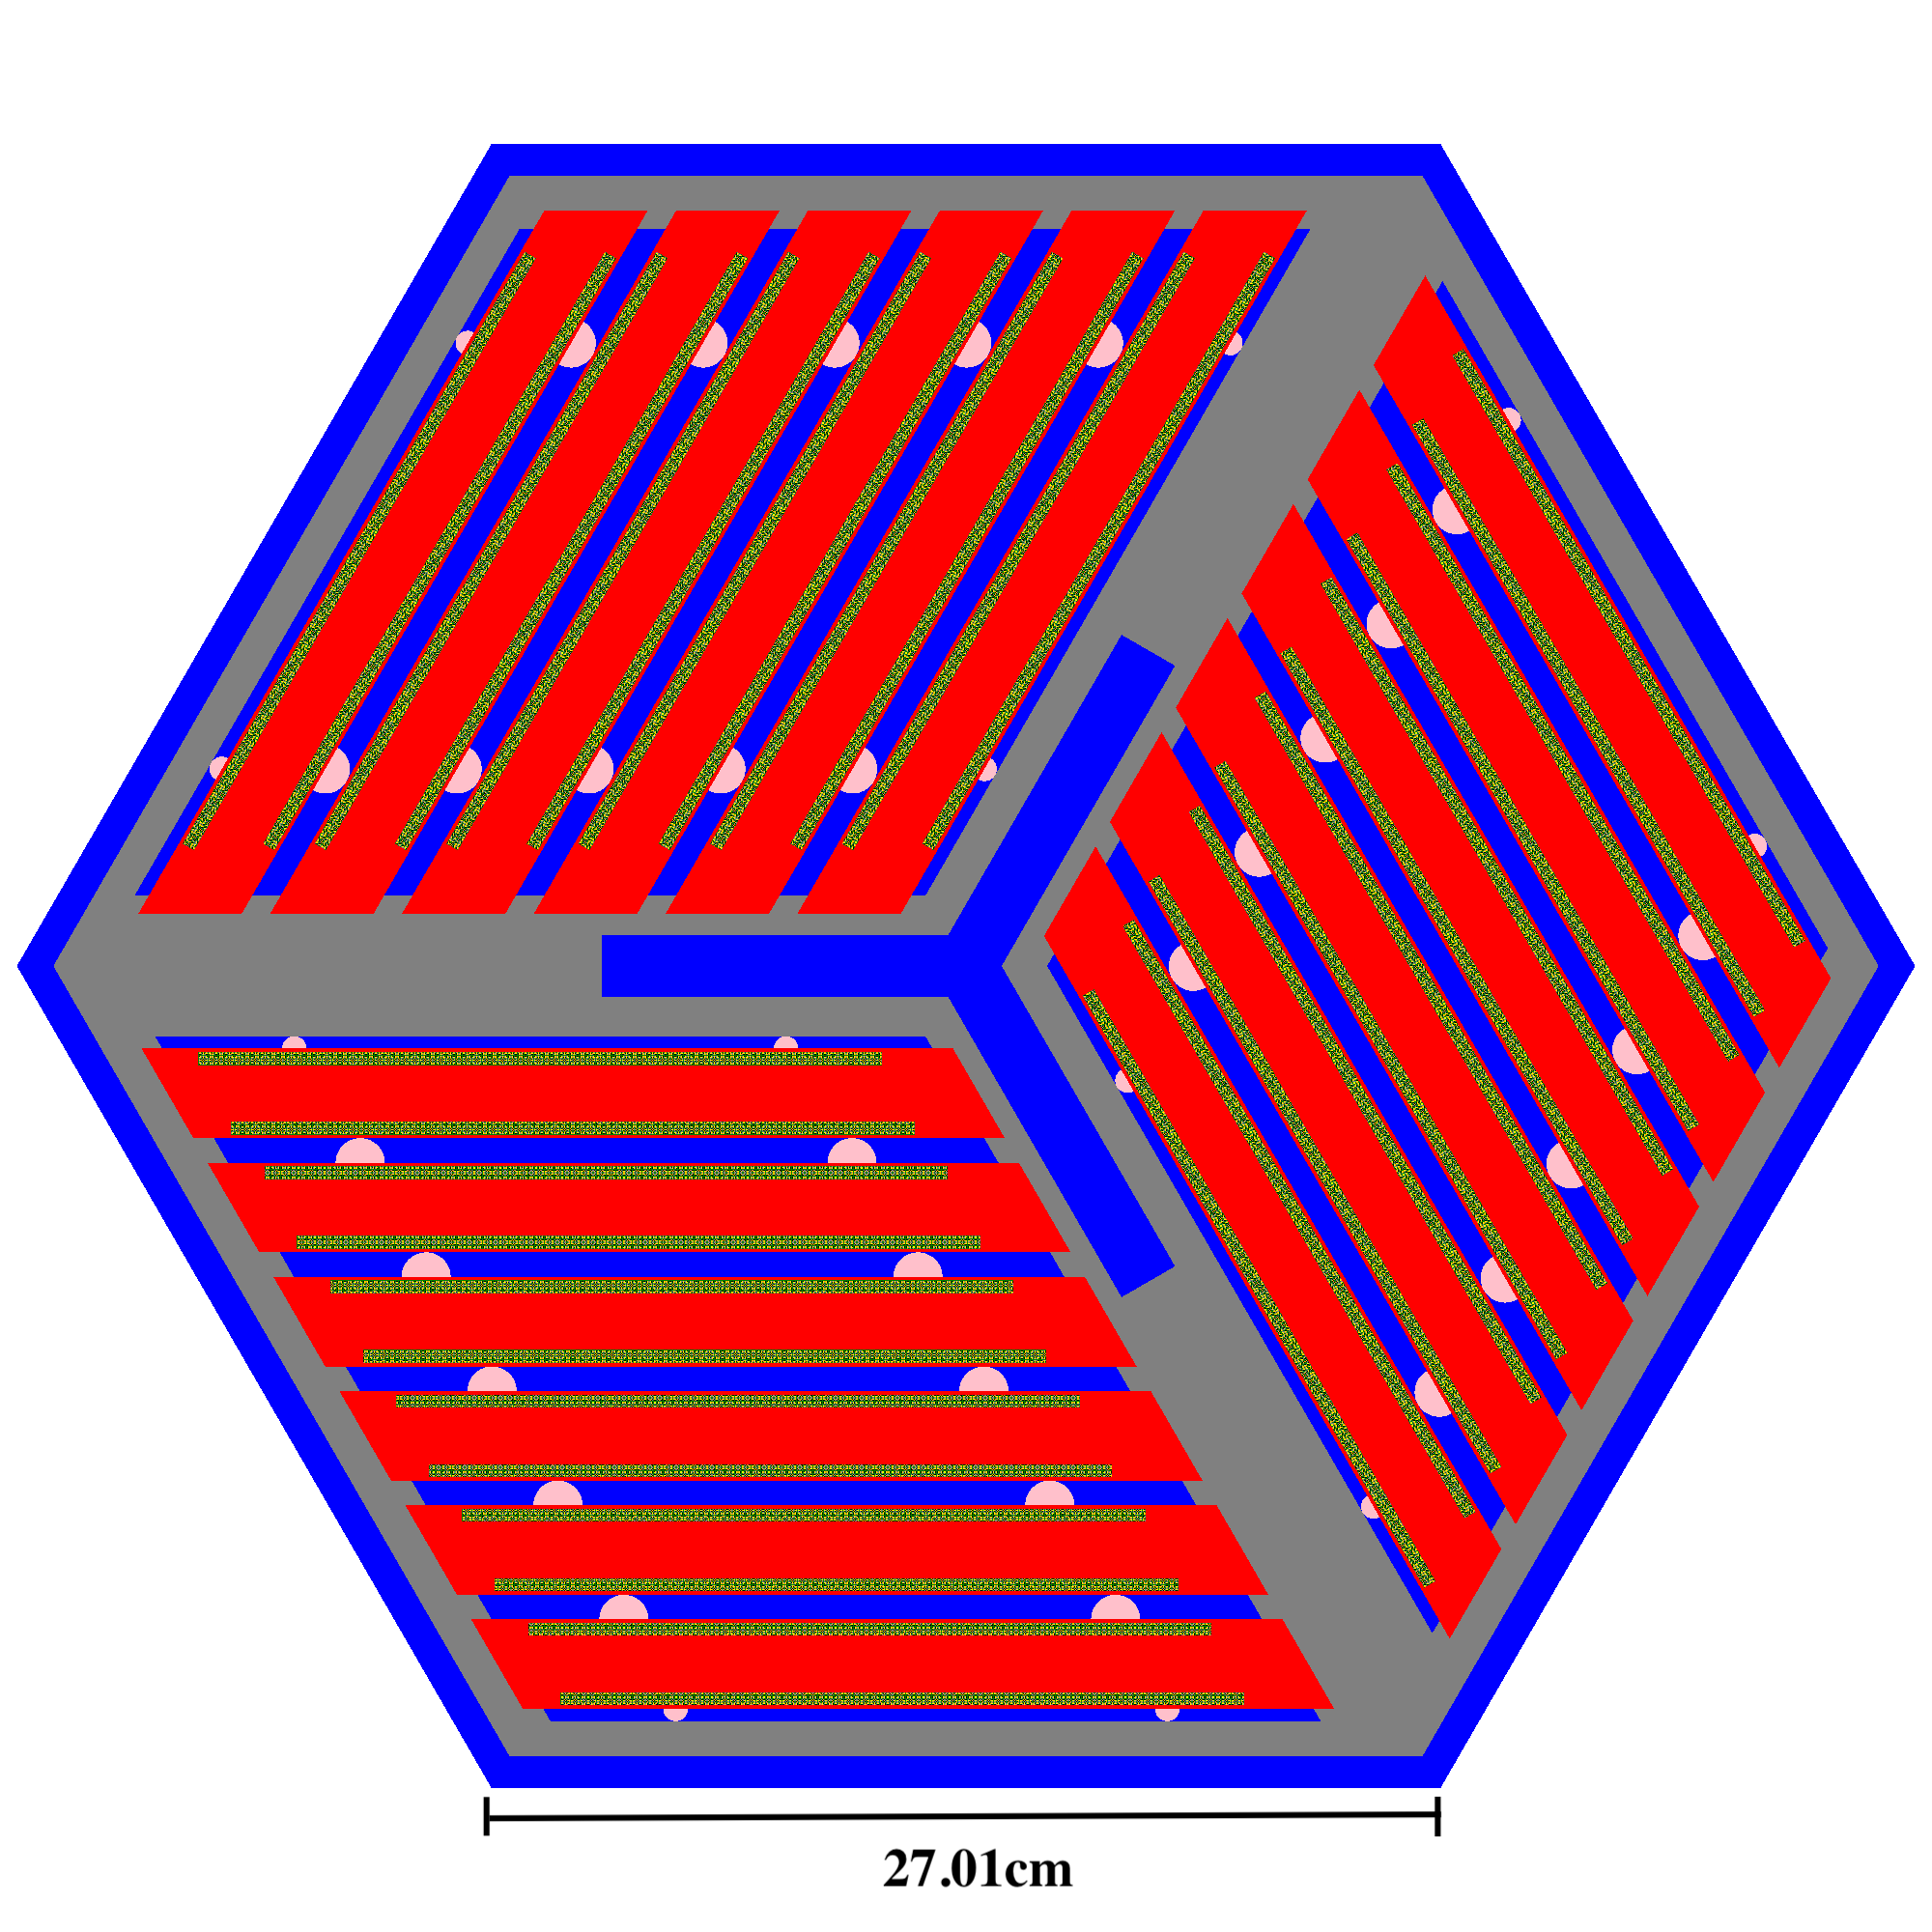
\includegraphics[width=0.49\linewidth]{../docs/figures/ahtr-fuel-element.png} 
        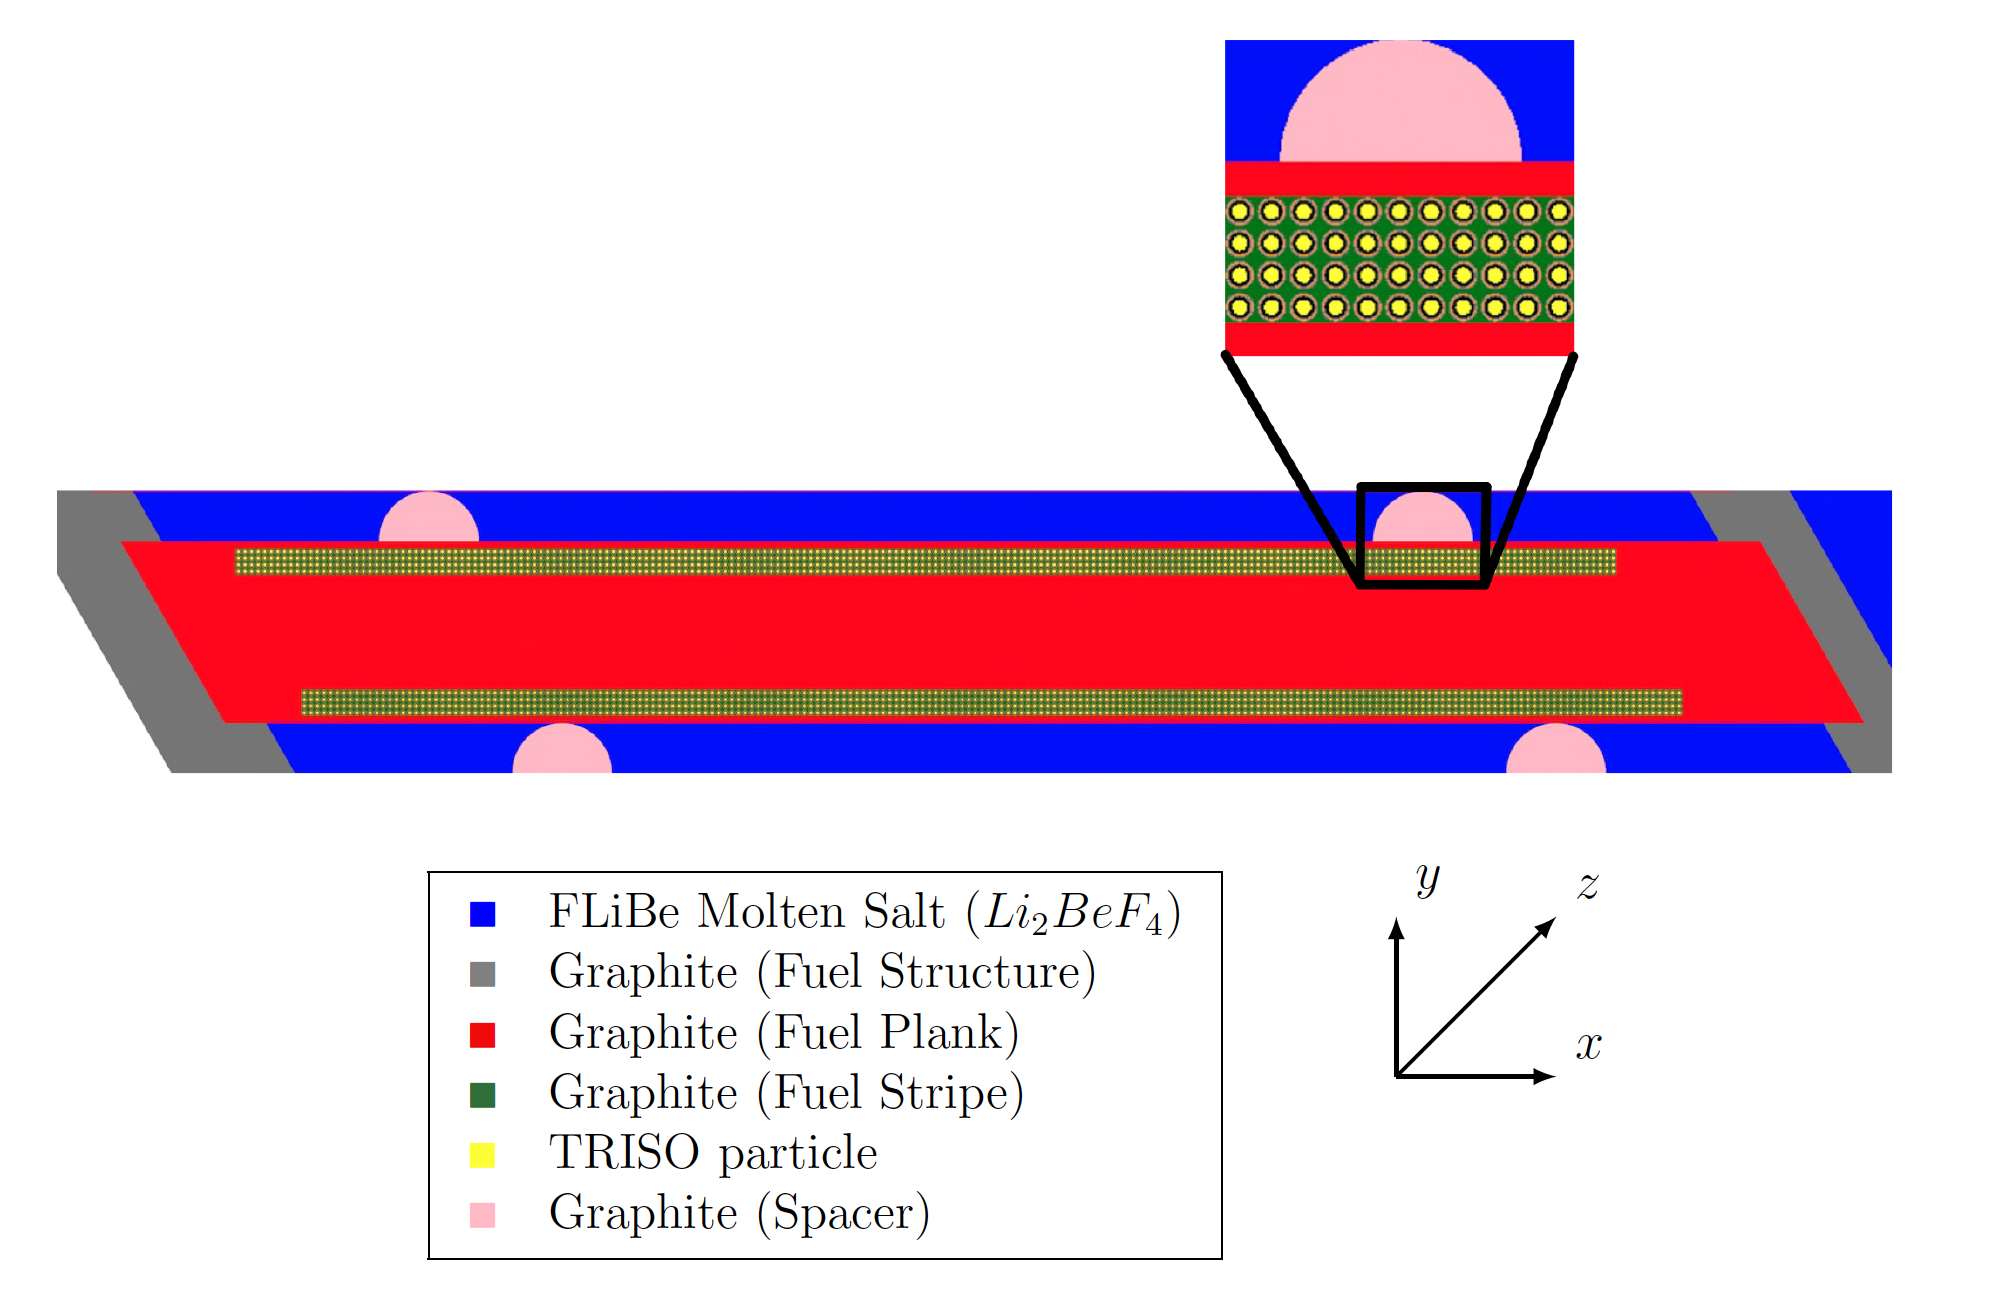
\includegraphics[width=0.49\linewidth]{figures/ahtr-plank.png}
        \caption{AHTR fuel assembly with 18 fuel plates arranged in 
        three diamond-shaped sectors, with a central Y-shaped and external channel 
        graphite structure.}
    \end{figure}
    \end{frame}

    \begin{frame}
    \frametitle{FHR Benchmark}
    \begin{itemize}
        \item The AHTR's fuel geometry's triple heterogeneity results in
        complex reactor physics and significant modeling challenges
        \item In 2019 the OECD-NEA initiated a FHR benchmark exercise. Its objective 
        is to identify the applicability, accuracy, and practicality of the latest 
        methods and codes to assess the current state of the art for FHR simulation 
        and modeling
    \end{itemize}
    \begin{figure}[]
        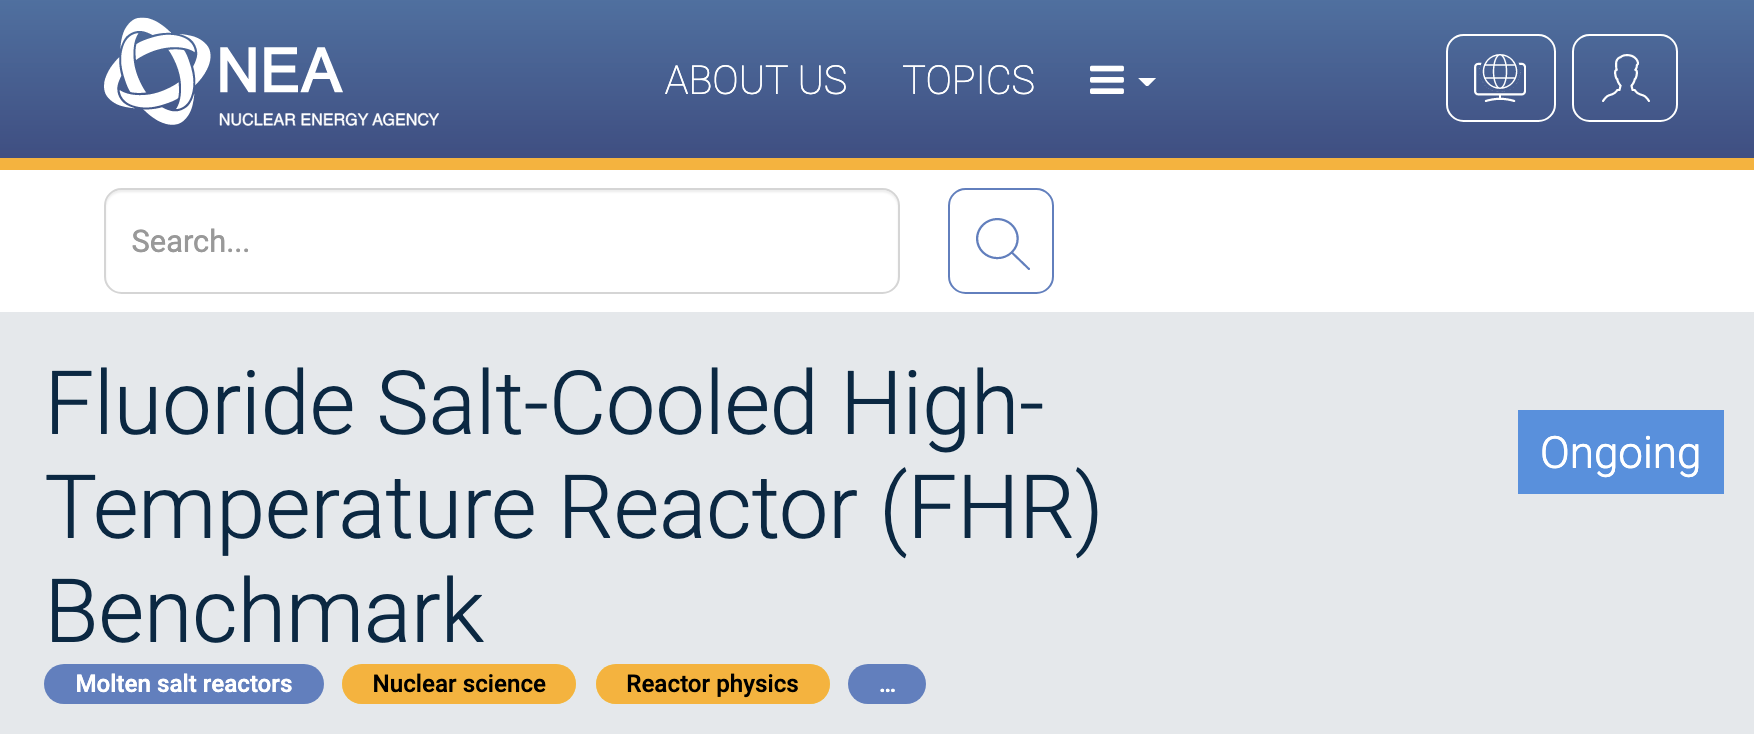
\includegraphics[width=0.7\linewidth]{figures/benchmark.png} 
        \caption{OECD NEA's FHR Benchmark \cite{petrovic_benchmark_2021}.}
    \end{figure}
    \end{frame}

\subsection{Objectives: AHTR Model Development}
    \begin{frame}
        \frametitle{Research Objectives: AHTR Model Development}
        \begin{block}{Technical Gap}
            The triple heterogeneity introduced by the geometrically complex 
            fuel assembly design makes accurate reactor physics simulations challenging. 
        \end{block}
        \begin{block}{Research Objectives: AHTR Model Development}
        \begin{itemize}
            \item Further our understanding of the AHTR design's complexities 
            through neutronics and thermal-hydraulics modeling
            \item Participate in the OECD-NEA's FHR Benchmark 
        \end{itemize}
        \end{block}
        \begin{block}{Link to Reactor Optimization for Non-conventional Designs}
        \begin{itemize}
        \item By participating in the benchmark, I ensure an accurate AHTR base model
        \item Thus, I can expect accurate answers for the optimized AHTR designs
        \end{itemize}
        \end{block}
    \end{frame}

% add some generative design lingoo
\subsection{Background: AHTR Optimization for Non-Conventional Designs}
\begin{frame}
    \frametitle{3D Printing a Nuclear Reactor?}
    \begin{block}{Impact of Additive Manufacturing Technology Advancements on 
        Reactor Design Optimization}
        \begin{itemize}
            \item Leveraging additive manufacturing enables us to surpass classical 
            manufacturing constraints and optimize for arbitrary geometries and parameters 
            such as non-uniform channel shapes, and inhomogeneous fuel distribution 
            throughout the core
            \item Wide-spread adoption of additive manufacturing methods in the nuclear industry 
            could drastically reduce reactor fabrication costs and deployment timelines 
            and improve reactor safety
            \item Fully benefitting from the new ability to 3D print reactor components 
            requires further research into reactor generative design optimization
          \end{itemize}
    \end{block}
  \end{frame}

  \begin{frame}
    \frametitle{Generative Reactor Design Optimization}
    Generative design is a design exploration process. Designers input design goals and 
    constraints into the generative design software. The software explores all the possible 
    permutations of a solution, quickly generating design alternatives. 
    It tests and learns from each iteration what works and what doesn't.
  \end{frame}

  \begin{frame}
    \frametitle{Evolutionary Algorithm Optimization}
    \begin{block}{Evolutionary Algorithms for Reactor Design Optimization}
    \begin{minipage}[c]{0.6\textwidth}
        \begin{itemize}
            \item We can leverage evolutionary algorithm optimization to 
            explore the large design space enabled by 3D printing to find global 
            optimal designs
            \item Evolutionary algorithms have proven successful in optimizing 
            multi-objective problems as they can find solutions at the global 
            optimum and can be run in parallel
            \item Evolutionary algorithms imitate natural selection to evolve solutions 
            \end{itemize}
  \end{minipage}\hfill
  \begin{minipage}[c]{0.4\textwidth}
    \centering
    \begin{figure}
      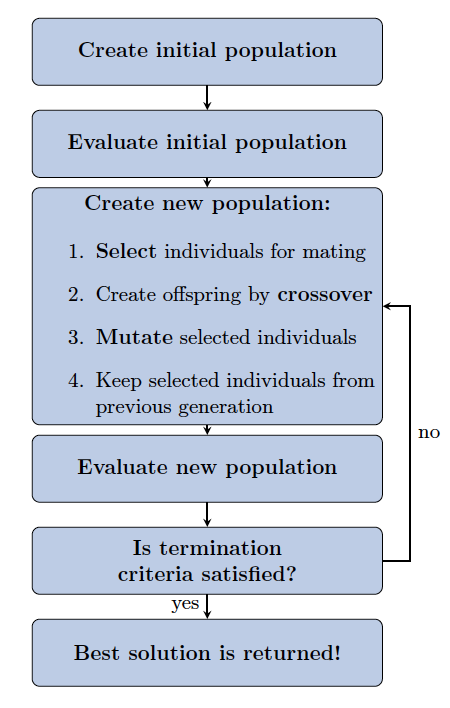
\includegraphics[width=0.8\linewidth]{figures/ea-flow.png} 
      \caption{Evolutionary algorithm flow \cite{renner_genetic_2003}. }
    \end{figure}
  \end{minipage}
  \end{block}
  \end{frame}

\subsection{Objectives: AHTR Optimization for Non-Conventional Designs}
\begin{frame}
    \frametitle{Research Objectives: AHTR optimization for non-conventional designs}
    \begin{block}{Technical Gap}
      \begin{itemize}
        \item Optimization tools for generating new reactor designs enabled by
        3D printing do not exist
        \item Reactor optimization for non-conventional geometries and parameters 
        has not been done 
      \end{itemize}
    \end{block}
    \begin{block}{Research Objectives: AHTR optimization for non-conventional designs}
        \begin{itemize}
            \item Develop an open-source tool that applies evolutionary algorithms 
            with established nuclear software to optimize reactor design
            \item Demonstrate successful application of the optimization tool 
            for single and multi-objective AHTR optimization of 
            non-conventional geometries and fuel distribution
        \end{itemize}
    \end{block}
  \end{frame}

\subsection{Summary}
\begin{frame}
    \frametitle{Research Objectives: Summary}
    \textbf{Additive manufacturing has the potential to radically transform reactor design.}
    \begin{block}{Research Objectives: AHTR Model Development}
        \begin{itemize}
            \item Further our understanding of the AHTR design's complexities 
            through neutronics and thermal-hydraulics modeling
            \item Participate in the OECD-NEA's FHR Benchmark
        \end{itemize}
    \end{block}

    \begin{block}{Research Objectives: AHTR optimization for non-conventional designs}
        \begin{itemize}
            \item Develop an open-source tool that applies evolutionary algorithms with established 
            nuclear software to optimize reactor design
            \item Demonstrate successful application of the optimization tool 
            for single and multi-objective AHTR optimization of 
            non-conventional geometries and fuel distribution
        \end{itemize}
    \end{block}
\end{frame}